\chapter{Project Cost Management}

Cost management is concerned with estimating, job control and data collection. The following are some techniques which are used to generate outputs such as cost management plans and cost requirements are as follows. 
\begin{enumerate}
\item Plan Cost Management
\item Estimate Costs
\item Determine Budget
\item Control Costs
\end{enumerate}

\section{Planning Cost Management}

Planning for cost management is a important part of cost management. Planning cost from the beginning will ensure accurate time and cost estimates. Expert judgement and experience is essential when managing and controlling project costs through a Cost Management Plan and Project Charters. 

A Cost Management Plan includes:
\begin{enumerate}
\item Units of measure
\item level of precision 
\item level of accuracy
\item Organisational procedures link
\item Control thresholds
\item Rule of performance measurement
\item Reporting formats
\item Process descriptions
\item Additional details
\end{enumerate}

\section{Budgeting}

When estimating cost in a project all risks and environmental and organizational process must be considered. A scope baseline is used to determine and prevent scope creep. An accurate and complete project scope statement, work breakdown structure and WBS dictionary are used to determine the project baseline.

\section{Realistic Targets}

Tools and techniques used to generate the work breakdown structures include:
\begin{enumerate}
\item Cost Aggregation 
\begin{itemize}
\item WBS are generated by grouping cost estimates into packages and those packages are then grouped into higher levels of the WBS.
\end{itemize}
\item Reserve Analysis
\begin{itemize}
\item It involves both the contingency reserves and the management reserves. 
\end{itemize}
\item Expert Judgement
\begin{itemize}
\item Mathematical models to predict total project cost are used to reconcile with with any funding limitations. A cost baseline,funding requirements and determined expenditures are now generated form the previous processes.
\end{itemize}
\end{enumerate}

\section{Cost Control}

There must be constant updates made to the project cost plans and any changes to the cost baseline must be updated. These changes are done through Cost forecasts and Change Requests and constantly documented and updated. 
Another technique used to measure project performance is Earned Value Management. This technique integrates scope time and cost date which is determined form the baseline. The following information is input into the EVM on a regular basis.

\begin{enumerate}
\item Planned Value(PV)
\item Actual Cost (AC)
\item Earned Value(EV)
\item Schedule Variances (SV)
\item Cost Variance (CV)
\item Schedule Performance Index(SPI)
\item Cost Performance Index(CPI)
\end{enumerate}

\begin{figure} [H]
\begin{center}
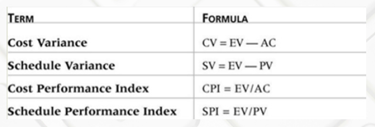
\includegraphics[scale=0.7]{evm.png}
\caption{EVM}
\label{fig:evm}
\end{center}
\end{figure}